\documentclass{examen}

\begin{document}
\modulo{Planificacion y administracion de redes.}
\pregunta{Explica qu� es una VLAN y para qu� sirve}{1}
\pregunta{�Qu� ocurre con las direcciones IP de una red cuando alguien dice pasar de no tener una VLAN a s� tenerla?}{0.5}
\pregunta{Observa la red de la figura. Escribe los comandos necesarios para crear VLANs y los subinterfaces asociados de acuerdo a la pertenencia a las VLAN que aparece en el gr�fico.}{5}

\pregunta{Asigna las direcciones IP, m�scaras y gateways que sean necesarios para que todo funcione. Crea tambi�n los comandos necesarios para conseguir lo siguiente:
\begin{itemize}
\item{Se desea que el tr�fico de las redes 80.24.118.0/24 entre al router pero no entre a la red.}
\item{Todas las m�quina aceptan la entrada de tr�fico ping pero el router no permitir� la salida de las respuestas.}
\item{Se permite el acceso desde el interior a la red 172.16.0.0/16}
\end{itemize}
.}{3.5}
\begin{figure}[h]
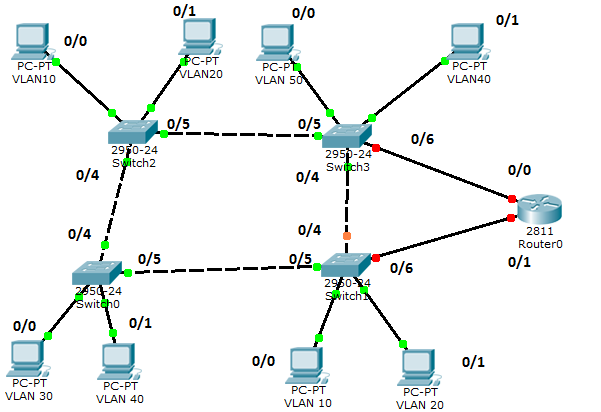
\includegraphics[scale=1]{examen-img/vlan.png}
\end{figure}
\end{document}
